\usetikzlibrary{calc}

\definecolor{DarkPink}{rgb}{0.55, 0.05, 0.37}

\newcommand*{\GridSize}{3}

\newcommand*{\ColorCells}[1]{% #1 = list of x/y/color
  \foreach \x/\y/\color/\text in {#1} {
    \node [fill=\color, draw=none, thick, ,minimum size=1cm] 
      at (\x-.5,\GridSize+0.5-\y) [text=white] {\text};
    }%
}%

\tikzset{near start abs/.style={xshift=1cm}}
%%%%%


%\listfiles
\scalebox{0.38}{ %%% scale it
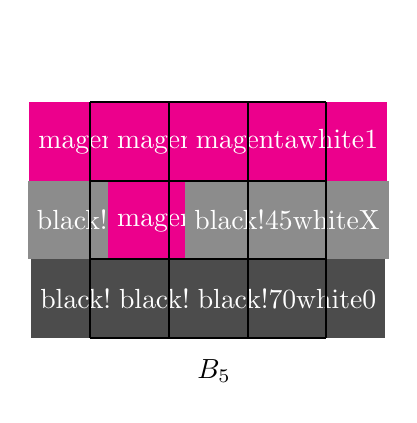
\begin{tikzpicture}
    \begin{scope}[thick,local bounding box=name]
    

         \fill[black!70](0,0) rectangle (\GridSize,\GridSize);
         \ColorCells{
         1/1/magenta/1, 2/1/magenta/1, 3/1/magenta/1,
         1/2/black!45/X, 2/2/magenta/1, 3/2/black!45/X,
         1/3/black!70/0, 2/3/black!70/0, 3/3/black!70/0
         }
        \draw (0, 0) grid (\GridSize, \GridSize);
        \draw (0.575,-0.7) node[above,near start abs] {$B_5$}; 
        \draw [->, draw=white,opacity=0] (1.1,3.5) -- node [above=0.8cm] {\textcolor{white}{invisible}} (1.3,1.8);
    \end{scope}
\end{tikzpicture}
} %%% case